% -*- mode: fundamental -*-

% ****************************************************************

\chapter{Pending (to be written): Fife}

\markboth{Ch \arabic{chapter}: Pending (DRAFT)}{\copyrightnotice}

\setcounter{page}{1}
% \renewcommand{\thepage}{\arabic{page}}
\renewcommand{\thepage}{\arabic{chapter}-\arabic{page}}

\label{ch_Fife_Pending}

% ****************************************************************

This is a place-holder chapter with a TODO list of pending possible
topics to be written.

In the Fife CPU, on the other hand, each of the yellow boxes
represents a ``stage'' and the black arrows represent messages sent
from one stage to another.  Each stage is itself an infinite loop,
consuming incoming messages and producing outgoing messages.  Thus,
while the Decode state is working on the first instruction, the Fetch
stage is already working on the second instruction, and so on.  There
is a sequence of instructions in this pipeline, advancing on every
``tick''.  A pipelined CPU also needs some additional state to manage
interactions between multiple instructions in the pipeline, such as
``epochs'', ``scoreboards'' and ``store-buffers'' (see
Figure~\ref{Fig_Instr_Exec_w_FIFOs}).


Figure~\ref{Fig_Instr_Exec_w_FIFOs} annotates the abstract execution
algorithm in Figure~\ref{Fig_Instr_Exec} with some specifics for the
pipelined implementation in Fife.
\begin{figure}[htbp]
  \centerline{\includegraphics[width=6in,angle=0]{ch030_RISCV_Design_Space/Figures/Fig_Instr_Exec_w_FIFOs}}
  \caption{\label{Fig_Instr_Exec_w_FIFOs}Pipelined interpretation of RISC-V instructions (same as Fig.~\ref{Fig_Instr_Exec})}
\end{figure}
In particular:
\begin{tightlist}

  \item Each of the yellow boxes is now itself a \emph{process}.  Each
    yellow box is an infinite loop that consumes data from input FIFOs
    and produces data on output FIFOs.  All yellow boxes run
    concurrently, which is how we get pipelined behavior.

  \item Pipelining requires that the Fetch unit fetches the ``next''
    instruction before it even knows what the current instruction is
    (it could be a BRANCH or a JAL/JALR which transfers control to a
    different PC that is not PC+4.  Fetching the instruction, and
    executing it, could result in a exception in which case, again,
    the ``next'' instruction will be at the PC for the trap handler,
    not the current PC+4.

    We may choose to respond to an external interrupt in which case,
    again, the ``next'' instruction will be at the PC for the
    trap/interrupt handler, not the current PC+4.

    As a result, we may fetch a ``wrong-path'' instruction. The
    \verb|epoch| register is for correcting wrong paths.

  \item Pipelining implies that an instruction reaching the RR step,
    and needing to read register $J$ may have to wait for an older
    instruction that is further down the pipe that has not yet
    completed to write a value into register $J$.  The
    \verb|scoreboard| is for dealing with this.

  \item Instructions may attempt to write to memory. The {\tt store
    buffer} holds these updates until we can deterimine whether the
    instruction is a wrong-path instruction or not.  If it's a wrong
    path instruction, we can discard the update, else commit it to
    memory.

  \item MMIO accesses may not be ``memory-like''.  A LOAD can have a
  side effect; a STORE may have side-effects more than just writing a
  value, such as starting a motor or launching a rocket!  Finally, a
  STORE to address $A$ followed by a LOAD from address $A$ may not
  return the same value.  For such accesses, the ``execute DMem''
  stage must defer the access until later when we are sure it is not a
  wrong-path instruction.

\end{tightlist}

\begin{figure}[htbp]
  \centerline{\includegraphics[width=6in,angle=0]{Figures/Fig_Fife_Retire}}
  \caption{\label{Fig_Fife_Retire}Actions in the ``Retire'' stage of Fife}
\end{figure}

\hdivider

% ****************************************************************

\section{Fife: pipelined execution}

Fife: Basic concepts of pipelined execution of instructions, {\ie}
pipelined implementation of the abstract algorithm of
Figure~\ref{Fig_Instr_Exec}.

Fife: parallel execution pipes for ``Execute'' steps in
Figure~\ref{Fig_Instr_Exec_w_FIFOs}

\begin{tightlist}

  \item Dispatching to different pipes after Register-Read

  \item Results from ``Execute'' pipes may be ready in different order from dispatch.

  \item   Tagging each pipe so ``Retire'' stage can retire in-order
\end{tightlist}


% ****************************************************************

\section{PC-prediction (control speculation)}

PC-prediction
\begin{itemize}
  \item The need for at least a minimal PC-prediction in Fetch stage:
        for many instructions, next-PC may not be known until deep in
        the pipeline; if so, what should Fetch do in the meantime?

    \begin{itemize}

      \item for conditional-branches (BRANCH) and jumps (JAL and
            JALR), next-PC is not known until ``Control'' step of the
            pipe.  What should Fetch do in the meantime?

      \item If there is a trap, next-PC changes from the normal next-PC.

        \begin{itemize}

          \item An instruction-fetch may trap, which we will discover
                only in memory-response arriving at the Decode stage

          \item The decode stage may find that the fetched
                ``instruction'' is not a legal instruction.  This
                causes a trap.

          \item An instruction may trap in the Execute stage ({\eg},
                LOAD/STORE/AMO may trap in memory access)

        \end{itemize}
    \end{itemize}

  \item The simplest predictor: PC+4

  \item Handling mispredictions: epochs, carrying epochs on
        instructions, discarding wrong-epoch.  How many epochs are
        needed?

  \item More advanced predictors
\end{itemize}

% ****************************************************************

\section{Register read/write hazards in Fife}

Scoreboards, scoreboard management, stalling-while-scoreboard busy.

Brief discussion of bypassing?

% ****************************************************************

\section{Speculative vs. non-speculative memory ops}

``Execute Memory Ops'' stage is always speculative (because of
mispredictions, and because older instructions in other pipes may
trap).

\begin{tightlist}
  \item Need for store-buffer and final commit/discard from Retire-stage
  \item Mem-system performs store only in store-buffer
  \item Retire stage sends commit/discard message to store-buffer.
        Discuss: do we need 'discard' messages, or are 'commit' messages enough?
\end{tightlist}

What about MMIO?

\begin{tightlist}
  \item LOADs may have side-effects
  \item LOADs may not be idempotent
  \item STOREs may have side-effects in addition to value stored
  \item LOAD may not return most-recently stored value
\end{tightlist}

So, these cannot be done speculatively, {\ie} in ``Execute Memory
Ops'' stage.

\begin{tightlist}

  \item 'Execute Memory ops' stage defers the request by sending it
    back as another kind of 'response'

  \item Retire step performs it once we know it is non-speculative.
\end{tightlist}

% ****************************************************************

\section{Fife: CSRs}

\begin{tightlist}
\item CSRRxx are read-modify-write operations
\item CSRRxx access may not be memory-like (side-effecting reads, read
      may not return last written value,
\item ... (a bit like MMIO issues)
\end{tightlist}
Hard to pipeline, so execute in Retire stage, as FSM.

CSRRxx instructions should be rare, so FSM exec does not affect overall performance.

% ****************************************************************

\section{Fife: Interrupts}

Sample for interrupts in Retire stage, fix up CSRs and and redirect.

Retire stage already has infra for CSR update and redirection, so this
is a small incremental change.

% ****************************************************************
